\documentclass[conference]{IEEEtran}
\IEEEoverridecommandlockouts
\usepackage{cite}
\usepackage{amsmath,amssymb,amsfonts}
\usepackage{algorithmic}
\usepackage{graphicx}
\usepackage{textcomp}
\usepackage{xcolor}
\usepackage{float}
\usepackage{rotating}
\usepackage{listings}

% Configuration for prompt code blocks
\lstset{
    basicstyle=\ttfamily\scriptsize,
    breaklines=true,
    breakatwhitespace=true,
    frame=lines,
    captionpos=b,
    keepspaces=true,
    showspaces=false,
    showstringspaces=false,
    aboveskip=1em,
    belowskip=1em
}

\def\BibTeX{{\rm B\kern-.05em{\sc i\kern-.025em b}\kern-.08em
    T\kern-.1667em\lower.7ex\hbox{E}\kern-.125emX}}

\begin{document}
\sloppy

\title{AquaLLM: Adaptive Large Language Model Agents for Autonomous Aquaculture Management\\}

\author{
\IEEEauthorblockN{Phu Leon Hoang}
\IEEEauthorblockA{\textit{Tickle College of Engineering} \\
University of Tennessee, Knoxville\\
Knoxville, TN\\
phoang5@vols.utk.edu}
}

\maketitle

\begin{abstract}
\normalfont
This report investigates the application of Large Language Models (LLMs) as autonomous decision-making agents for managing a biologically-inspired aquaculture simulation. The novelty of this work lies in adapting memory-driven reflection and tool-augmented reasoning from LLM agents to the complex, stochastic domain of environmental management. The proposed system, AquaLLM, utilizes a cognitive architecture where the agent observes pond states, reflects on past actions, and leverages external tools to optimize policies for Largemouth Bass (\textit{Micropterus salmoides}). By balancing survival rates, fish health, and strict budgetary constraints over multi-generational timelines, the agent successfully navigates the exploration-exploitation tradeoff. Ablation studies demonstrate that memory, planning, and tool-use are critical for preventing ecological collapse and maintaining economic viability in chaotic simulated environments.
\end{abstract}

\begin{IEEEkeywords}
Large Language Models, Embodied Agents, Agent-Based Modeling, Aquaculture, Particle Swarm Optimization
\end{IEEEkeywords}

\section{Introduction}

\subsection{Project Goal}
Aquaculture operations are highly dynamic environments that require constant monitoring and optimization to maximize fish yield while adhering to strict economic budgets. Poor management can quickly lead to disastrous consequences, including pathogen outbreaks, eutrophication, and intracohort cannibalism. The overarching goal of this project is to develop an intelligent, automated management system capable of optimizing resource distribution---specifically food, probiotics, and oxygen---for Largemouth Bass.

\subsection{Research Question}
The primary research question investigated in this paper is: Can an embodied Large Language Model (LLM) agent, equipped with environmental feedback, memory, and analytical tools, effectively optimize a complex, stochastic agent-based aquaculture model without relying on traditional mathematical optimizers?

\subsection{Topic Significance and Solution Architecture}
Standard mathematical models often fail to capture the localized, reactive nature of biological systems. This project solves the problem by deploying AquaLLM, an intelligent management framework powered by a local LLM. The new contribution is the adaptation of a cognitive agent architecture---incorporating multi-tiered reflection (checkpoints, warnings, and end-of-generation synthesis) and budget calculation tools---to iteratively optimize physical simulation parameters in real-time. This approach bridges the gap between natural language reasoning and bio-inspired computation, demonstrating that LLMs can adapt to physical resource management constraints.

\section{Related Work}
Agent-based modeling (ABM) is a standard method for understanding complex biological systems, allowing researchers to simulate factors like dissolved oxygen, fish shoal behavior, and spatial management strategies \cite{urbanova2023}. In the specific context of Largemouth Bass aquaculture, researchers have documented the severe environmental impacts of poor pond management in maintaining survival rates \cite{hou2023}.

Traditionally, optimization within these ABMs relies on heuristic algorithms like Evolutionary Algorithms or Particle Swarm Optimization. However, the advent of Large Language Models has introduced new paradigms for autonomous control. This project utilizes recent advancements in generative agents as a foundational reference. Park et al. (2023) demonstrated the efficacy of Generative Agents that maintain extensive memory streams to simulate believable interactive behavior \cite{park2023}. We adapt this memory-driven reflection specifically for environmental management, allowing the AquaLLM agent to ``remember'' past simulation days, detect patterns of biological decline, and autonomously adjust policies. 

Furthermore, our solution architecture draws heavy inspiration from Voyager, an open-ended embodied agent capable of exploring and mastering complex virtual worlds without human intervention \cite{wang2023}. Similar to Voyager, AquaLLM uses tools (such as mathematical budget calculators) and environmental feedback to iteratively optimize its control policy, evaluating resource expenditures against long-term fish survival.

\section{Technical Approach}

\subsection{Problem Domain and Rules}
The environment operates as a 3D simulated pond ($180 \times 85 \times 50$ units) containing a population of Largemouth Bass. The simulation is evaluated at 1-hour timesteps over a 30-day period. The overarching goal is to maximize a multi-objective Fitness score governed by specific weights. The agent must operate under a strict \$500 maximum budget. If the budget is exhausted early, or if all fish die due to starvation, oxygen depletion, or physical hazards, the simulation terminates.

\subsection{Core Simulation Engine Implementation}
The physical environment acts as a deterministic, biologically-inspired baseline. It is divided into distinct execution modules:
\begin{itemize}
    \item \textit{Entities and Physics:} The environment manages dynamic objects including consumable resources (food, probiotics, oxygen bubbles) and biological waste (fecal matter, dead fish). A strict eutrophication cycle is implemented: uneaten food and feces sink to the pond floor, decay into generic pollutants, and probabilistically transform into environmental hazards such as ammonia (NH3) clouds, disease zones, and parasites.
    \item \textit{Agent-Based Behavior:} Fish act as autonomous agents with internal physiological stats (health, fullness, immunity, oxygen) that decay every timestep. Movement is driven by a modified Particle Swarm Optimization (PSO) algorithm. Instead of seeking a mathematical global minimum, the PSO algorithm models the swarm intelligence of the fish to mimic a realistic aquaculture environment. Each fish dynamically computes its velocity vector based on a hierarchy of biological needs and environmental stimuli, such as schooling with peers, foraging for resources, and actively evading physical hazards and larger cannibalistic predators.
\end{itemize}

\subsection{Cognitive LLM Agent Architecture}
AquaLLM operates as a continuous ``Farm Manager'' loop interfacing with the physical simulation. The LLM does not control individual fish; rather, it controls the global distribution policy of food, probiotics, and oxygen. The system is compartmentalized into four core cognitive modules:

\subsubsection{Observation}
LLMs cannot natively process raw, continuous 3D coordinate data. The Observation module discretizes the continuous $180 \times 85$ pond space into a $3 \times 3$ localized semantic grid (e.g., \textit{Top-Left}, \textit{Center}, \textit{Bottom-Right}) to map hazard zones and fish distributions. It aggregates these raw numerical states into a natural language string. Crucially, it computes a quantitative ``warning points'' metric to alert the LLM to impending ecological crises. This score is calculated using weighted multipliers for severe events: for example, each dead fish adds 10 points, each infected fish adds 5 points, and large physical hazard zones add points scaling with their spatial radii.

\subsubsection{Tool}
LLMs notoriously struggle with exact arithmetic over long horizons. The Tool module integrates deterministic Python functions exposed to the LLM via JSON schemas. The primary tool, \texttt{calculate\_budget}, computes the exact 30-day cost of feeding and pumping schedules. A secondary tool, \texttt{compare\_day\_fitness}, mathematically compares the current day's Fitness against the exact same day in the previous generation. Because generative models occasionally hallucinate or misspell function names and parameters, this module utilizes a Levenshtein-distance fuzzy matching algorithm with an endurance of up to 2 characters to automatically correct spelling errors. Furthermore, if the LLM fails to invoke a valid tool, it is allowed up to 2 retry attempts before safely falling back to a ``do nothing'' protocol (rolling over the previous day's policy).

\subsubsection{Planning}
The Planning module provides the agent with Chain-of-Thought (CoT) reasoning capabilities. It processes the text outputs from the Observation and Memory modules to formulate localized rationales for resource distribution, enabling the agent to deduce cause-and-effect relationships (e.g., ``Ammonia is spiking and survival dropped; reduce food quantity to limit waste'') before generating a final policy payload. 

\subsubsection{Memory}
To prevent context window overflow over a 720-timestep simulation, the agent utilizes a dynamic Memory module. It records daily policies, observations, and fitness scores. To maintain token efficiency, a compaction algorithm triggers periodically, truncating older daily logs and replacing them with a dense statistical summary. This ensures the agent retains long-term historical trends while preserving exact semantic logs of the most recent days for immediate context.

\subsection{Premium Cognitive Features}
The following advanced capabilities are not isolated scripts, but rather emergent features that are only obtainable by successfully combining multiple base cognitive modules.

\begin{itemize}
    \item \textit{Multi-Tiered Reflection:} This mechanism requires the combination of the Memory and Planning modules. It allows the agent to synthesize compacted historical logs to establish stronger, evidence-based initial policies for subsequent generations, and to execute mid-generation course corrections during acute crises. Because it operates independently of external mathematical tools or localized text grids, Reflection remains active across the \textit{Full}, \textit{No Observer}, and \textit{No Tools} configurations.
    \item \textit{Early Quit (Proactive Abort):} This mechanism requires the exact combination of the Memory, Tool, and Planning modules. Starting from Generation 3, the agent can use the \texttt{compare\_day\_fitness} tool to mathematically evaluate its current trajectory against historical baselines fetched from Memory. If the current run is performing significantly worse, the Planning module can proactively trigger an ``Early Quit.'' When triggered, this mechanism seamlessly invokes an ``Early-Quit Reflection,'' guiding the LLM to analyze the failure and select a more robust initial policy to restart the generation with. To prevent infinite restart loops, the system strictly limits this to a maximum of 3 attempts. Because it does not strictly rely on semantic environmental text, this feature is obtainable in both the \textit{Full} and \textit{No Observer} configurations.
\end{itemize}

\subsection{Examined Options (Ablation)}
To rigorously evaluate the necessity of each module, several configurations were tested: 
\begin{itemize}
    \item \textit{Full:} All features enabled. This configuration unlocks all base modules and premium cognitive features.
    \item \textit{No Planning:} Zero-shot generation without CoT reasoning.
    \item \textit{No Memory:} An amnesic agent completely restricted from historical data access. Disabling this strictly disables any capacity for temporal reflection, end-of-generation synthesis, or historical fitness comparison.
    \item \textit{No Tools:} Agent must guess mathematical budget constraints (disabling the \texttt{calculate\_budget} and \texttt{compare\_day\_fitness} tools, thereby disabling the Early Quit feature).
    \item \textit{No Observer:} Agent receives raw JSON state dictionaries instead of semantic text.
    \item \textit{Minimal:} Baseline LLM with no cognitive scaffolding.
\end{itemize}

\section{Dataset and Implementation}

\subsection{Generative Dataset Domain}
This project fundamentally departs from traditional machine learning pipelines by completely eliminating the use of static, pre-recorded external datasets. In contrast, AquaLLM operates as an embodied agent within an open, continuous environment. The custom 3D physical simulation acts as a live, generative data engine. The ``data'' fed to the LLM consists entirely of the dynamic, stochastic interaction outcomes between the fish swarm and the agent's own resource management decisions. This closed-loop embodiment provides a chaotic testing ground to evaluate the LLM's capacity to adapt to evolving scenarios over a 30-day lifecycle.

\subsection{Hardware and Execution Environment}
The system architecture and simulation logic are written entirely in Python. The project is deployed using the Google Colab Pro for Students tier, allocated an NVIDIA H100 Tensor Core GPU. This hardware setup provides the critical CUDA acceleration necessary to compute parallel physics updates and execute local LLM generations with minimal latency.

\subsection{LLM Configuration and Context Limits}
The cognitive framework is powered by the Qwen2.5 family (7B and 72B parameter configurations) hosted directly on the Colab instance via the Ollama local inference server. A critical bottleneck is the context window. The 7B model has a hard limit of 32,000 tokens, while the 72B model expands this to 128,000 tokens. However, empirical testing revealed that tracking 30 simulation days demands approximately 400,000 to 500,000 tokens. Consequently, both models fundamentally overflow their context limit if unmanaged. The agent relies entirely on the Memory Compaction module to prevent fatal Out-Of-Memory (OOM) crashes.

\subsection{Robustness and Syntax Enforcement}
AquaLLM implements multiple layers of fallback enforcement:
\begin{itemize}
    \item \textit{Levenshtein Fuzzy Matching:} Automatically corrects hallucinated JSON keys during tool dispatch to the nearest canonical parameter.
    \item \textit{No Raw JSON Enforcement:} Extracts structured payloads from CoT prose, refusing malformed JSON blocks.
    \item \textit{Iterative Retry Loop:} Allows the agent up to 2 retry attempts when output is fundamentally unparseable.
    \item \textit{Ultimate Fallback (Policy Rollover):} Safely falls back to a ``do nothing'' state (rolling over the previous day's policy) if all retries fail.
\end{itemize}

\section{Experiments and Results Analysis}

\subsection{Experimental Setup}
The experiments were conducted over 5 distinct generations per configuration to measure the agent's ability to learn. The simulation initialized 50 fish per pond. The primary evaluation metric is Fitness, calculated based on the following weighted multi-objective formula:

\begin{equation}
\boxed{\text{Fitness} = 0.55 \cdot \text{Yield} + 0.33 \cdot \text{Saving} + 0.12 \cdot \text{Health}}
\end{equation}

\subsection{Cross-Model Overall Performance Comparison}
To establish a baseline of how model scale impacts management, Figure \ref{fig:cross_model} compares the ultimate Fitness achieved. While the 72B model outperforms the 7B model in complex configurations, the performance delta is not as impressive as the exponentially higher computational cost suggests. The 7B model proves surprisingly capable for base autonomous management, though the 72B model affords a slightly deeper understanding of multi-step biological causality.

\begin{figure}[H]
    \centering
    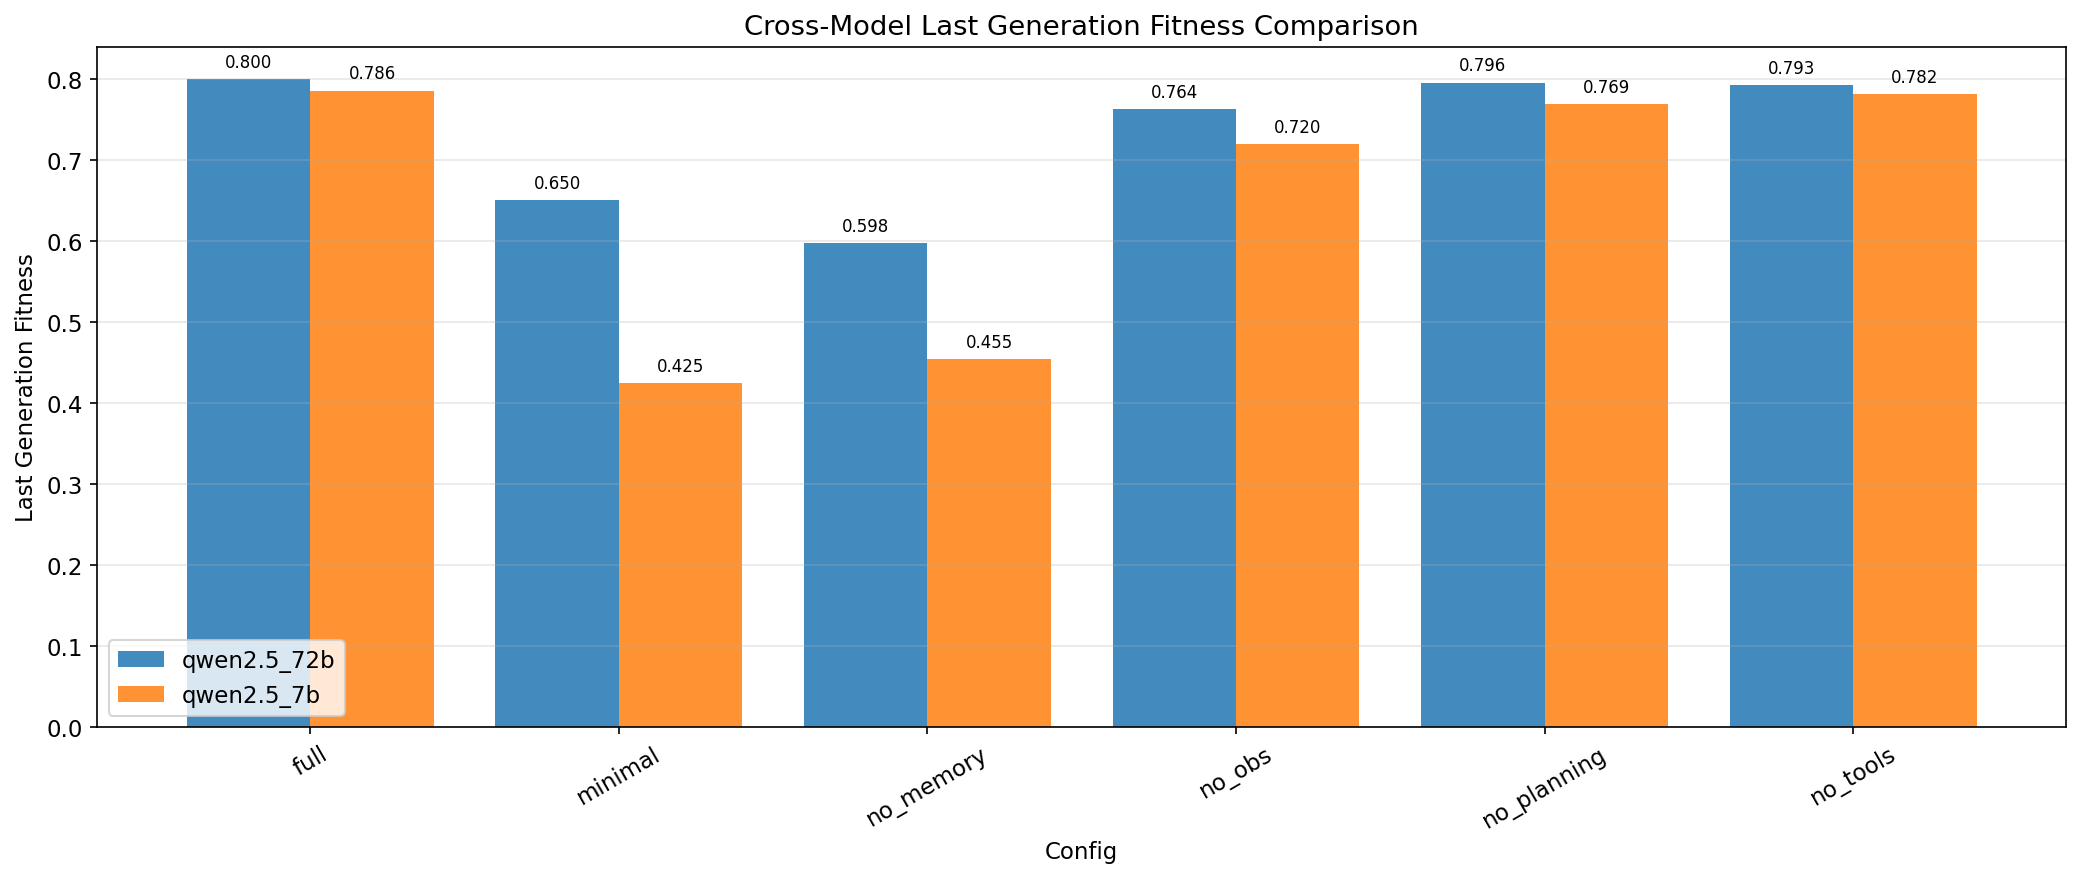
\includegraphics[width=0.85\linewidth]{../plots/comparison/cross_model_last_generation_fitness.png}
    \caption{Final Generation Fitness Comparison across all configurations (Qwen2.5 7B vs 72B).}
    \label{fig:cross_model}
\end{figure}

\subsection{Learning Curve: Fitness by Generation}
Tracking Fitness across 5 generations (Figures \ref{fig:fitness_gen_7b} and \ref{fig:fitness_gen_72b}) demonstrates the evolutionary capability of the architecture. For both models, the \textit{no\_memory} configuration shows a severe drop line. We believe this occurs because an amnesic agent cannot build a coherent temporal strategy, resulting in a failure to stabilize the environment across generations. While the 7B model exhibits a slow learning curve due to misinterpreting past failures, the 72B model demonstrates rapid stabilization through superior Chain-of-Thought abstraction.

\begin{figure}[H]
    \centering
    \begin{minipage}{0.48\textwidth}
        \centering
        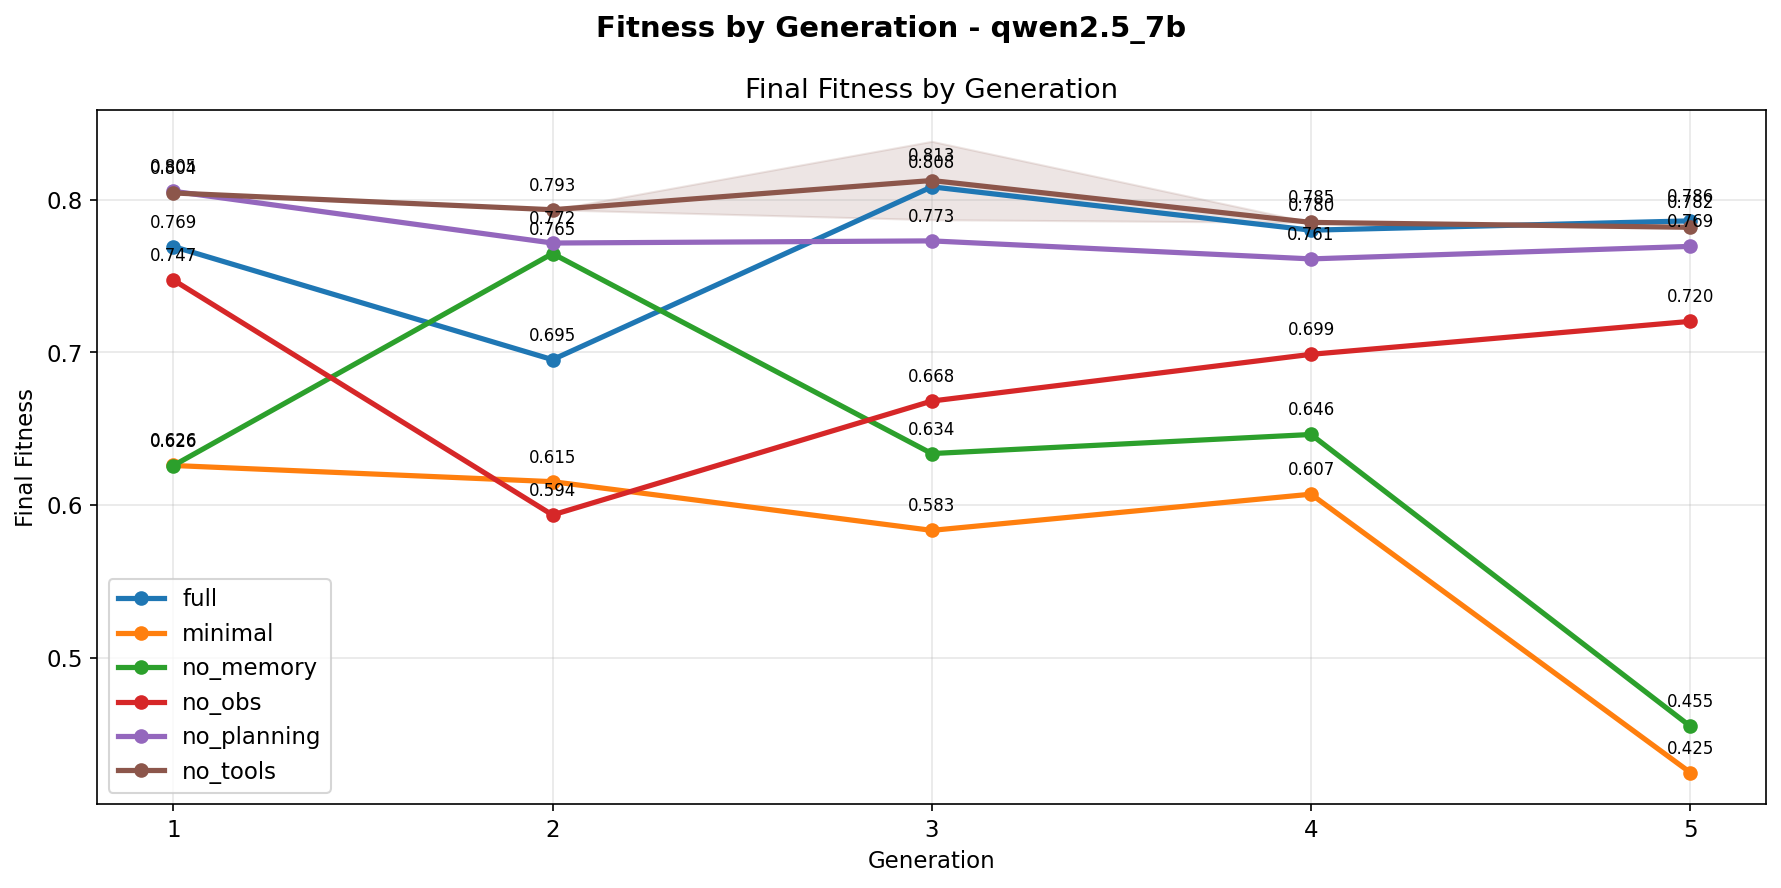
\includegraphics[width=\linewidth]{../plots/qwen2.5_7b/fitness_by_generation.png}
        \caption{Fitness by Generation (Qwen2.5 7B)}
        \label{fig:fitness_gen_7b}
    \end{minipage}\hfill
    \begin{minipage}{0.48\textwidth}
        \centering
        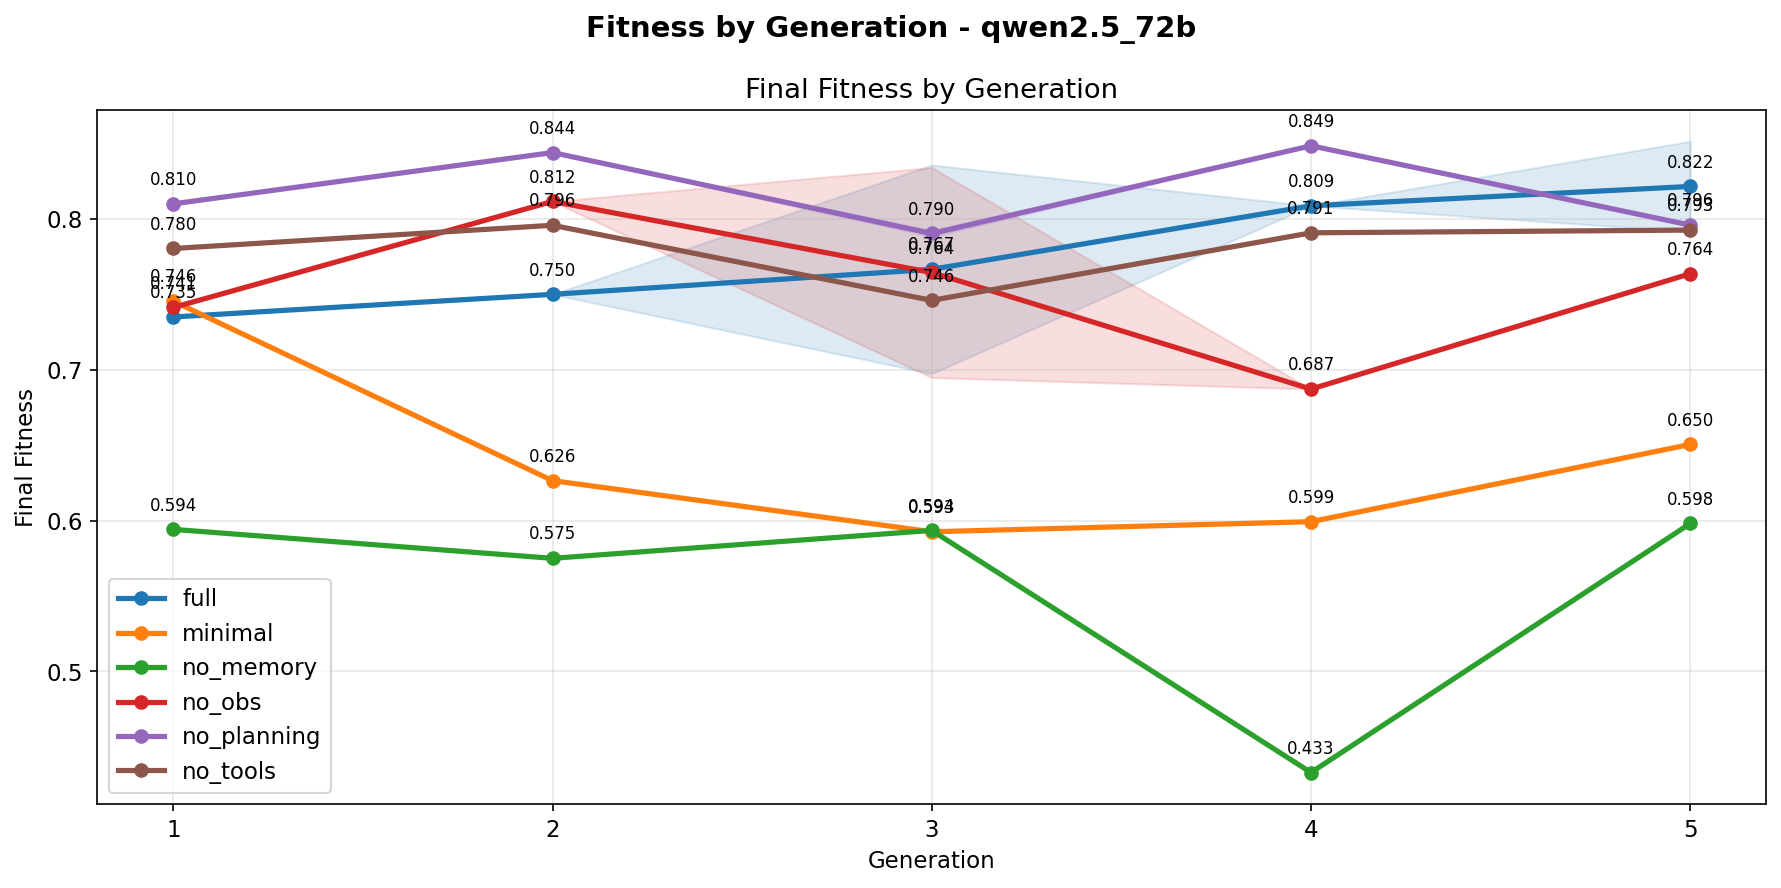
\includegraphics[width=\linewidth]{../plots/qwen2.5_72b/fitness_by_generation.png}
        \caption{Fitness by Generation (Qwen2.5 72B)}
        \label{fig:fitness_gen_72b}
    \end{minipage}
\end{figure}

\subsection{Final Generation Metrics}
Constituent metrics (Figures \ref{fig:last_gen_bars_7b} and \ref{fig:last_gen_bars_72b}) show that the 7B model often fails budget conservation when survival rates decline. In contrast, the 72B model clearly still struggles to understand how to Save, as indicated by its high spending. However, this spending is more useful than the 7B model's, as it helps the fish survive better and remain healthier. Crucially, the \textit{minimal} configuration performs significantly better than \textit{no\_memory}. This suggests a long-context issue: \textit{minimal} receives shorter context and thus less noise than \textit{no\_memory}, which still processes tool and planning logs without the benefit of reflection. This confirms that memory is the ultimately important factor in stabilization.

\begin{figure}[H]
    \centering
    \begin{minipage}{0.48\textwidth}
        \centering
        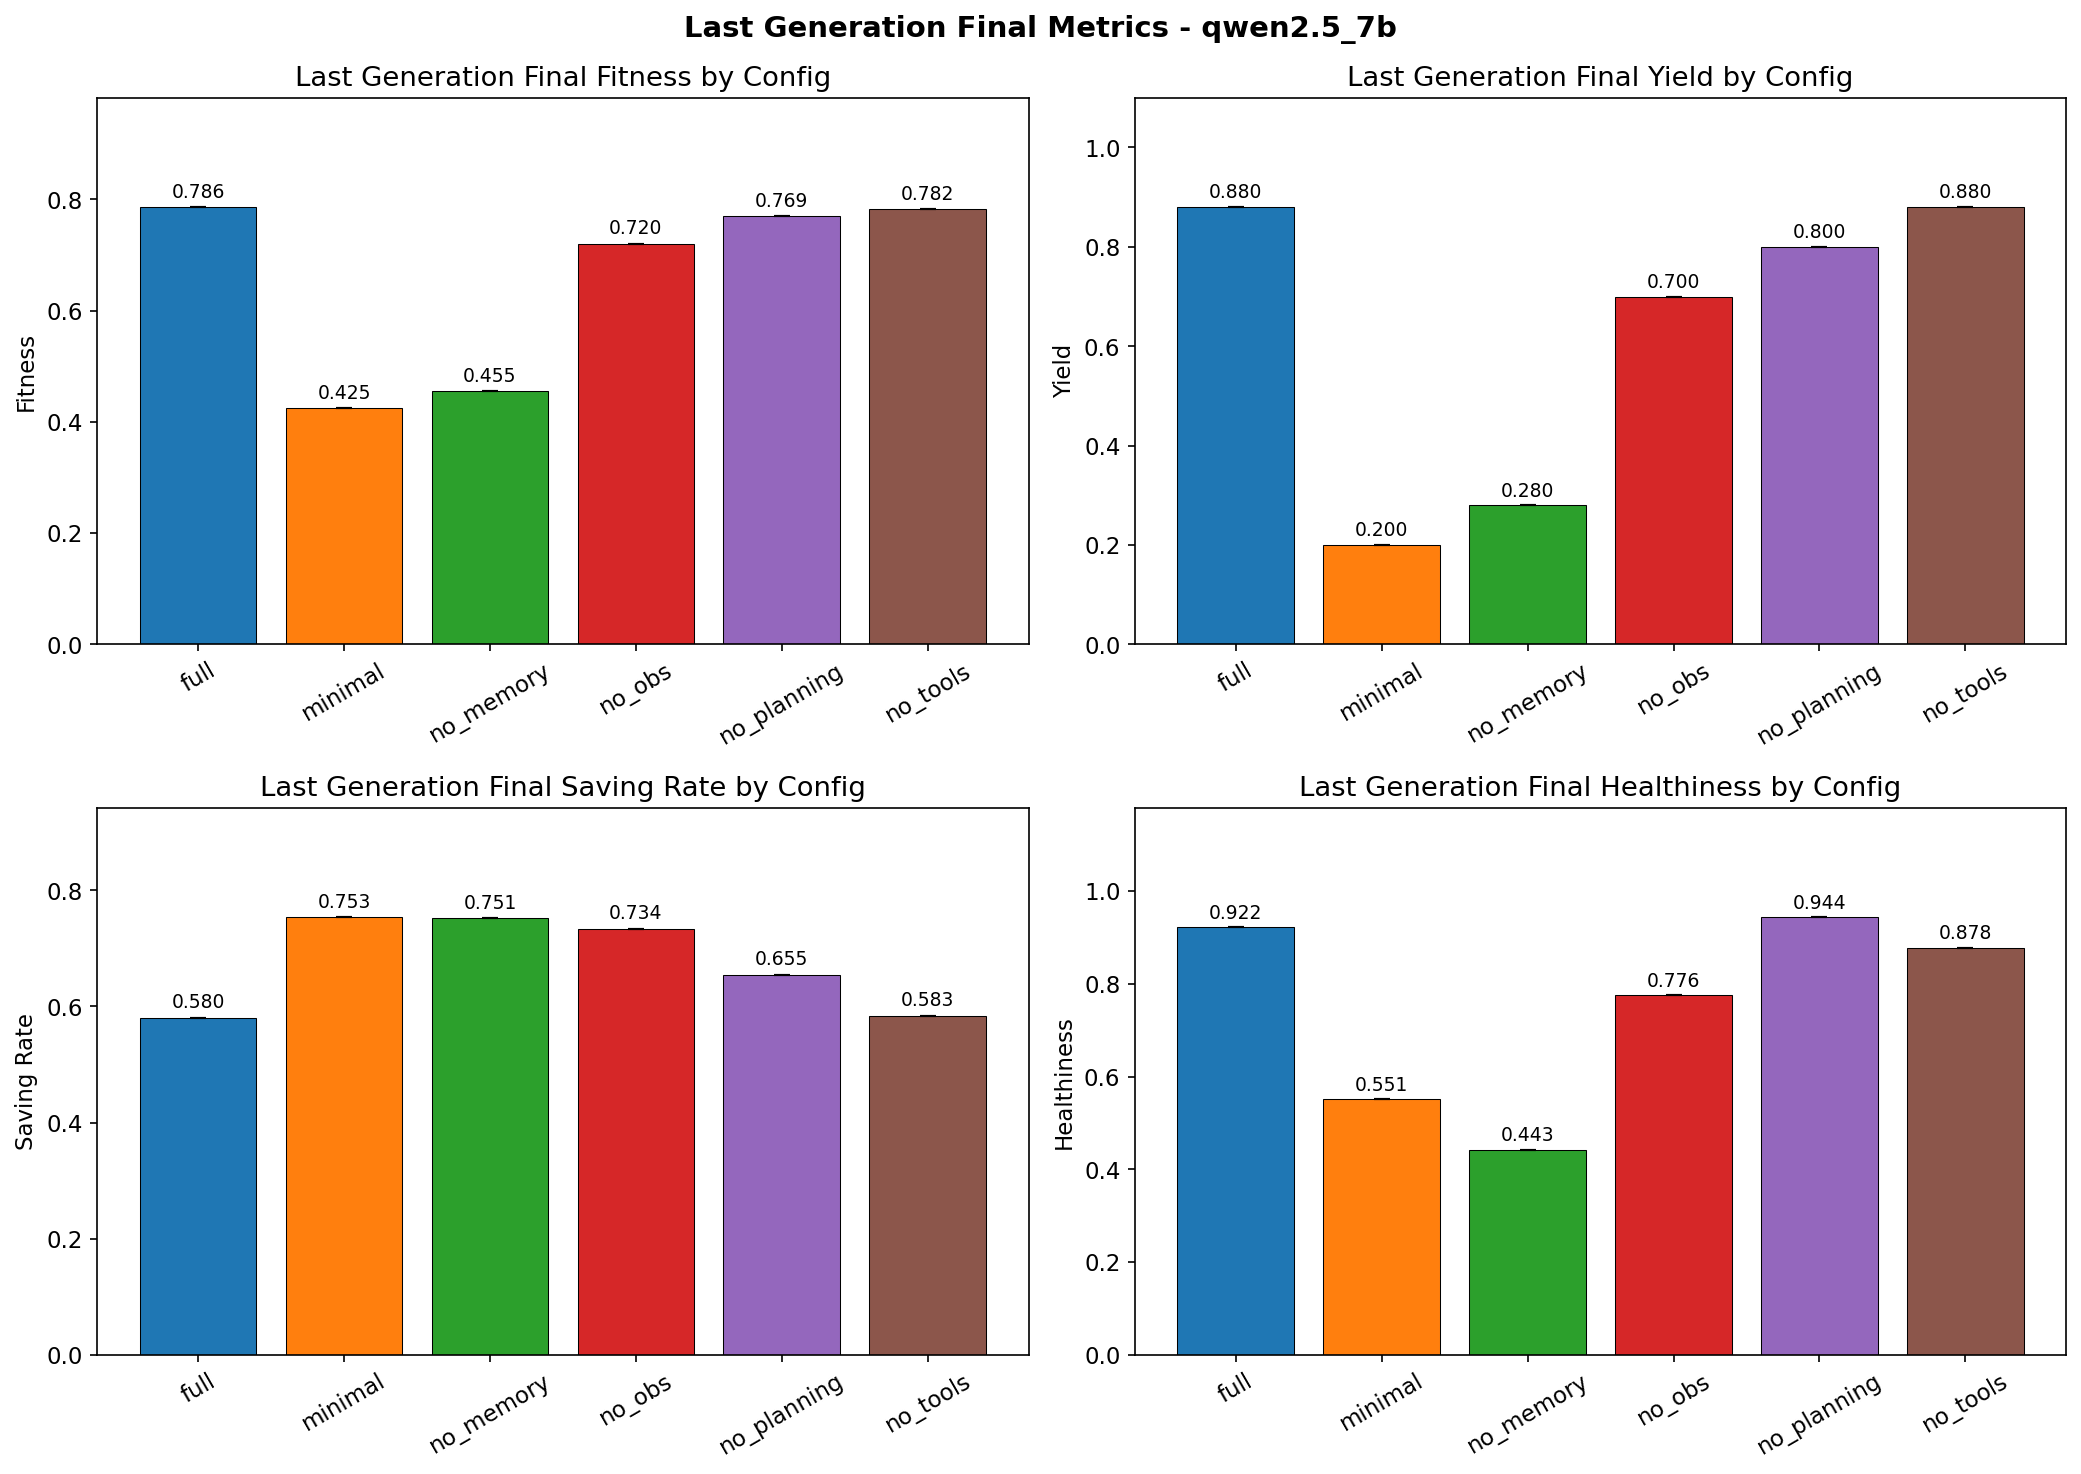
\includegraphics[width=\linewidth]{../plots/qwen2.5_7b/last_generation_bars.png}
        \caption{Final Generation Metrics (Qwen2.5 7B)}
        \label{fig:last_gen_bars_7b}
    \end{minipage}\hfill
    \begin{minipage}{0.48\textwidth}
        \centering
        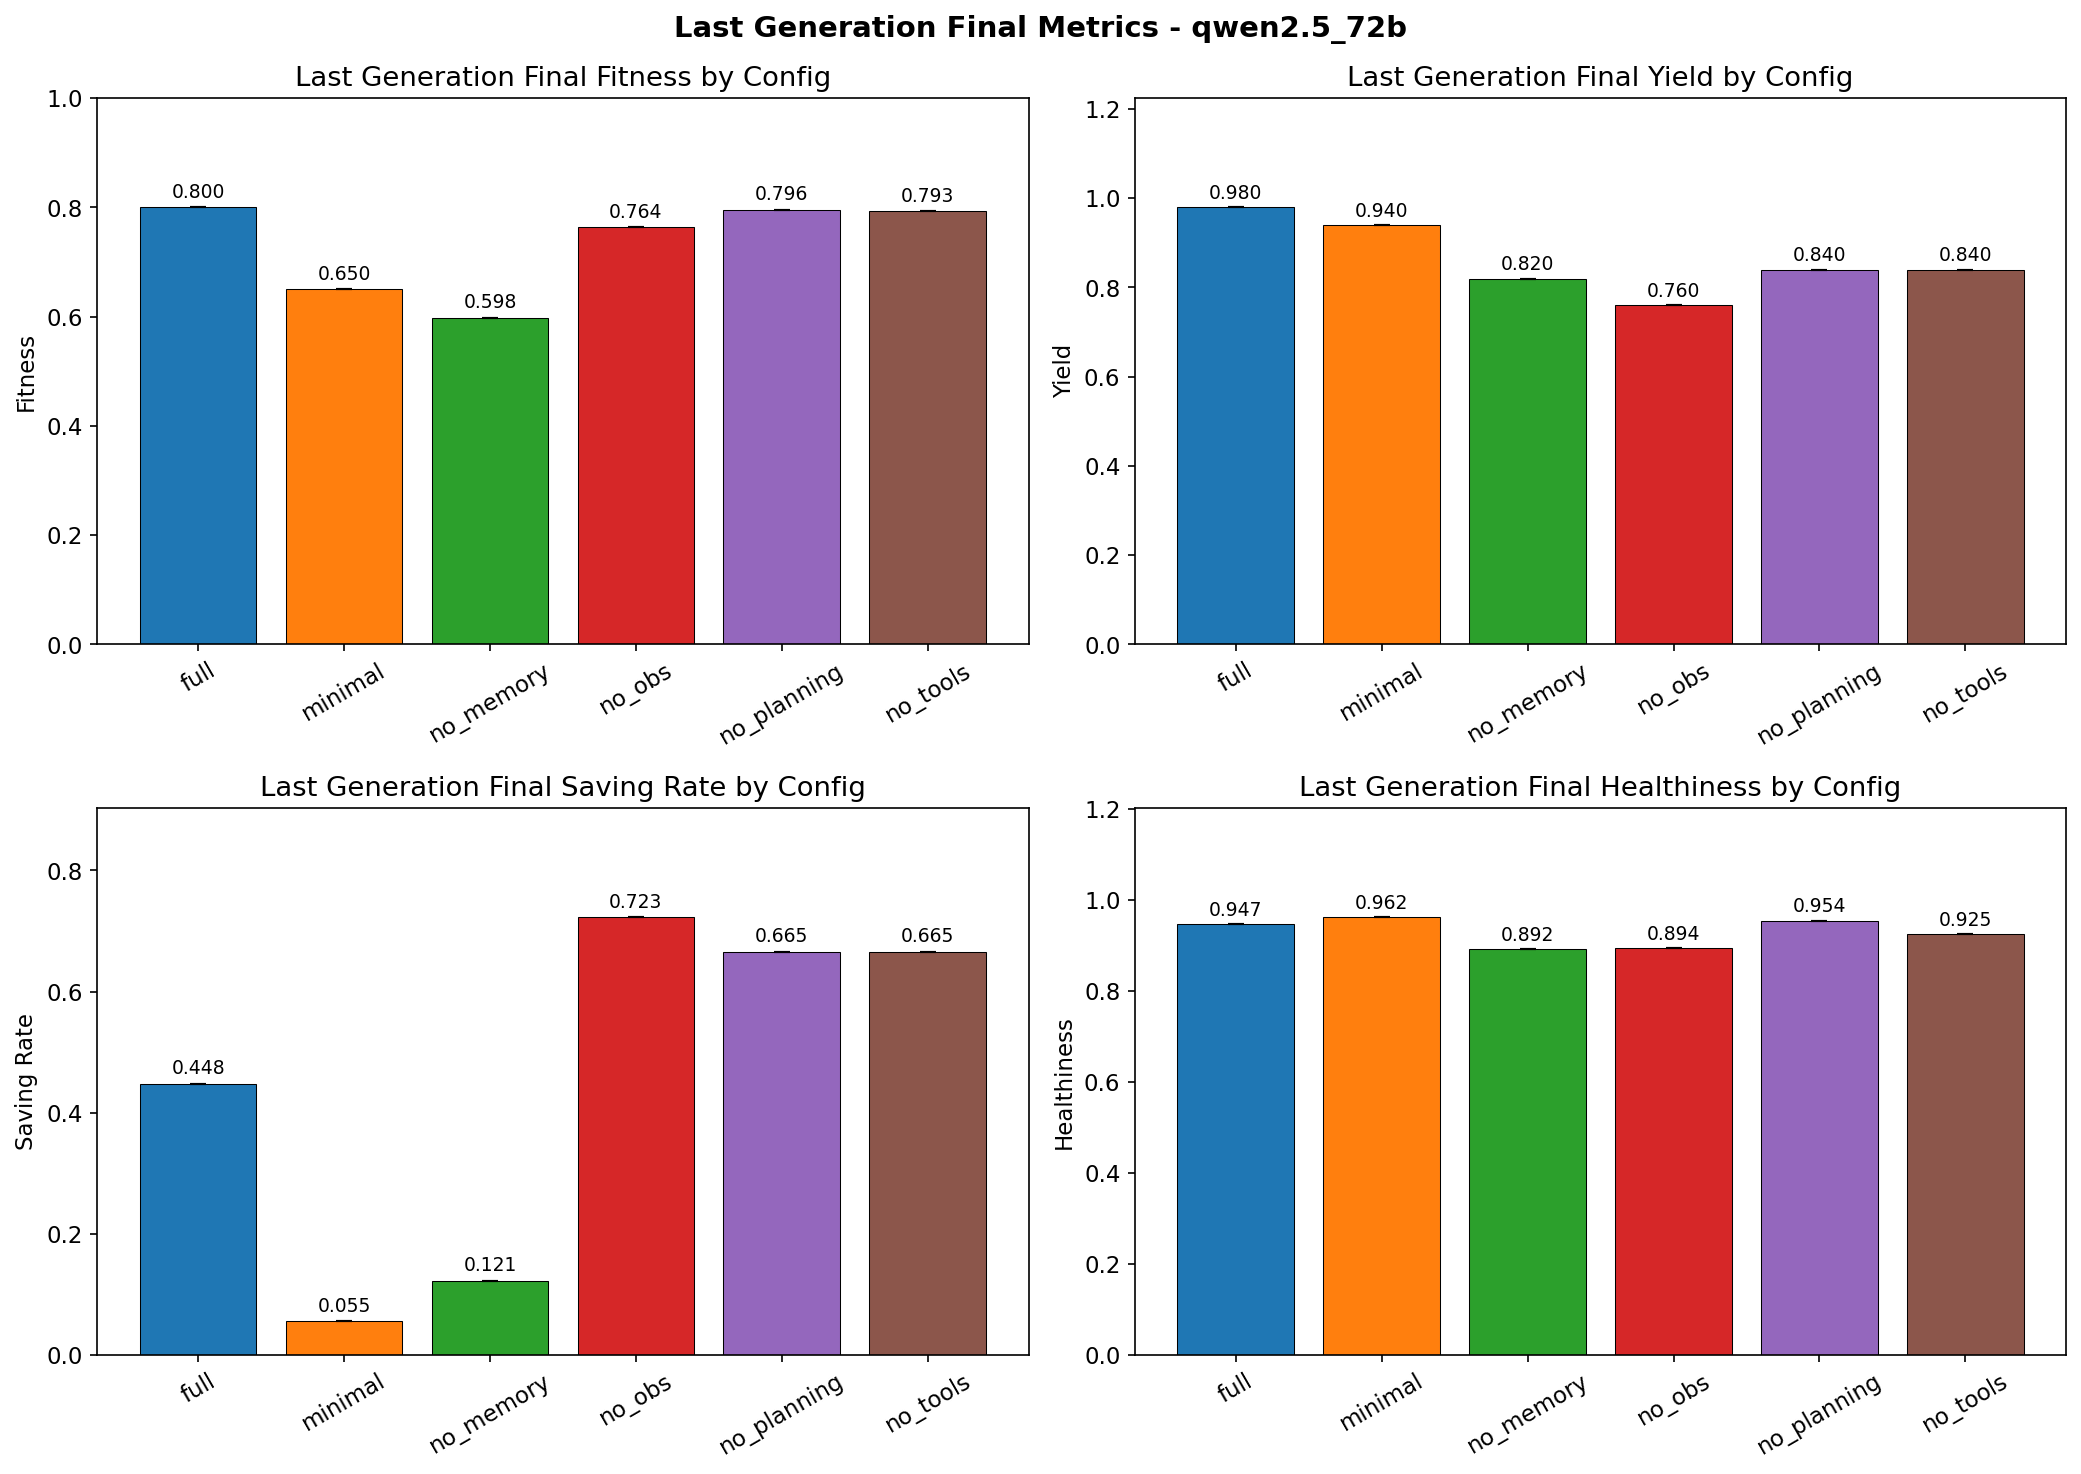
\includegraphics[width=\linewidth]{../plots/qwen2.5_72b/last_generation_bars.png}
        \caption{Final Generation Metrics (Qwen2.5 72B)}
        \label{fig:last_gen_bars_72b}
    \end{minipage}
\end{figure}

\subsection{Importance Heatmap}
The ablation heatmaps (Figures \ref{fig:heatmap_7b} and \ref{fig:heatmap_72b}) reveal the fragility of the models when ablated. \textit{No Memory} reliably triggers catastrophic failure in 7B Yield. While 72B exhibits stronger resilience, it still suffers in the Saving metric under the \textit{No Tools} ablation. This indicates that even at 72B, the model cannot accurately project compounding costs over 30 days without external tool grounding.

\begin{figure}[H]
    \centering
    \begin{minipage}{0.48\textwidth}
        \centering
        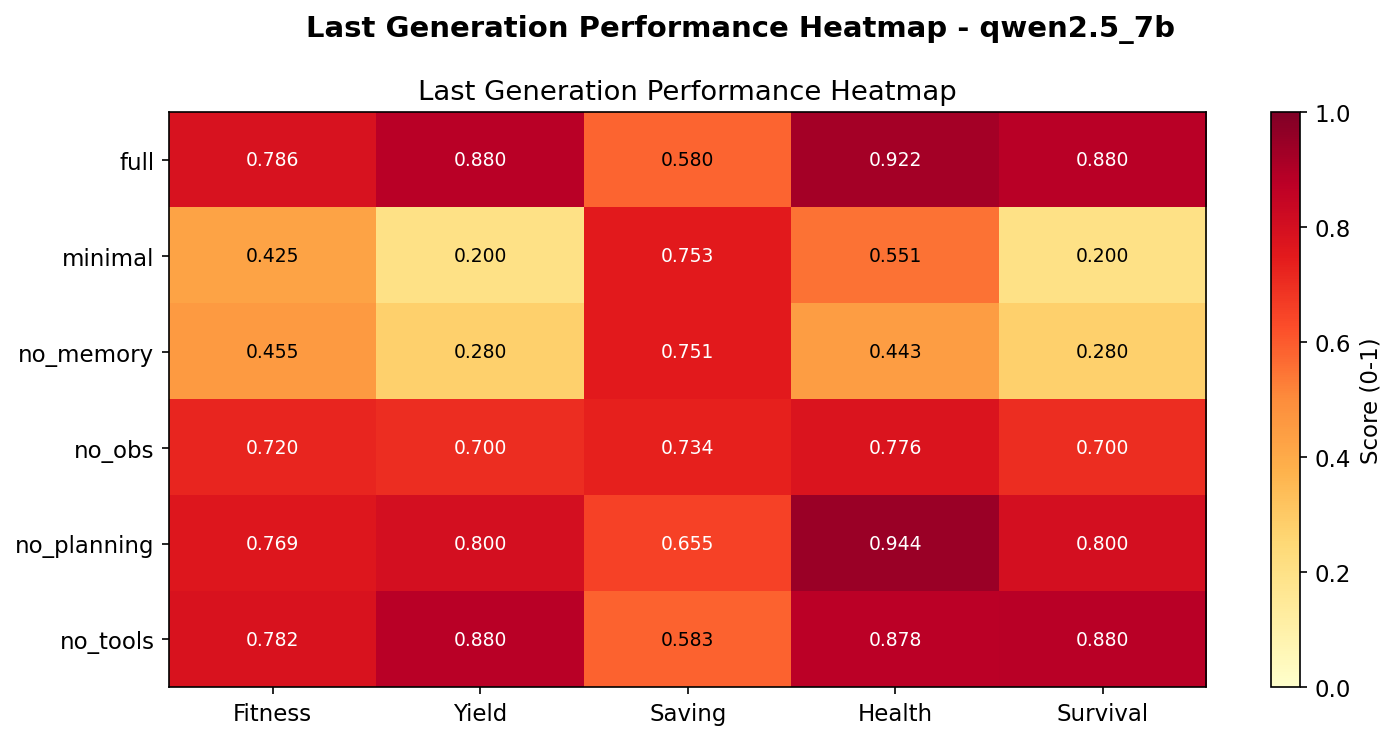
\includegraphics[width=\linewidth]{../plots/qwen2.5_7b/ablation_heatmap.png}
        \caption{Ablation Heatmap (Qwen2.5 7B)}
        \label{fig:heatmap_7b}
    \end{minipage}\hfill
    \begin{minipage}{0.48\textwidth}
        \centering
        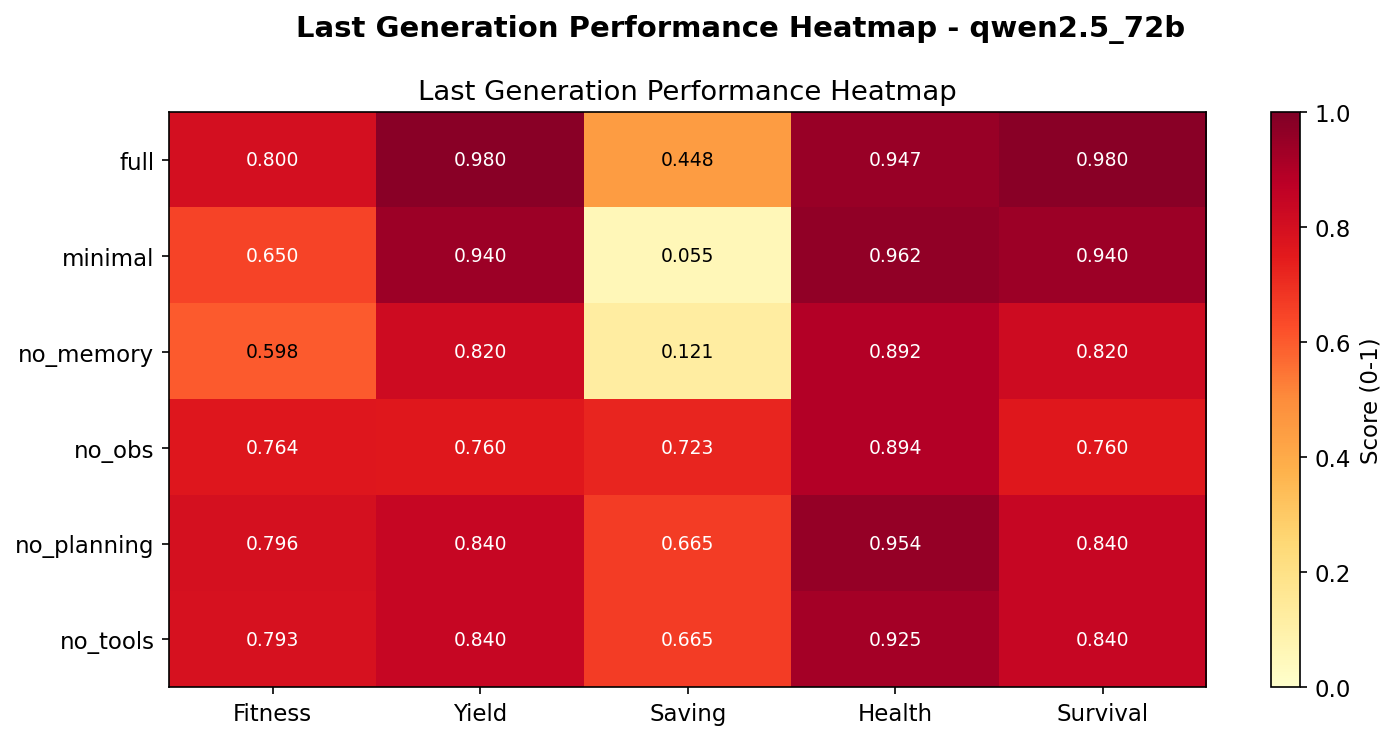
\includegraphics[width=\linewidth]{../plots/qwen2.5_72b/ablation_heatmap.png}
        \caption{Ablation Heatmap (Qwen2.5 72B)}
        \label{fig:heatmap_72b}
    \end{minipage}
\end{figure}

\subsection{Resource Management Trajectory}
The simulation trajectories (Figures \ref{fig:trajectory_7b} and \ref{fig:trajectory_72b}) show that both 7B and 72B models operating under the \textit{Full} architecture perform equally well, maintaining controlled depletion. Ablated configurations, however, exhibit sharp vertical drops—depleting the budget abruptly due to unchecked intervals or suffering massive mortality due to an inability to react to ammonia spikes.

\begin{figure}[H]
    \centering
    \begin{minipage}{0.48\textwidth}
        \centering
        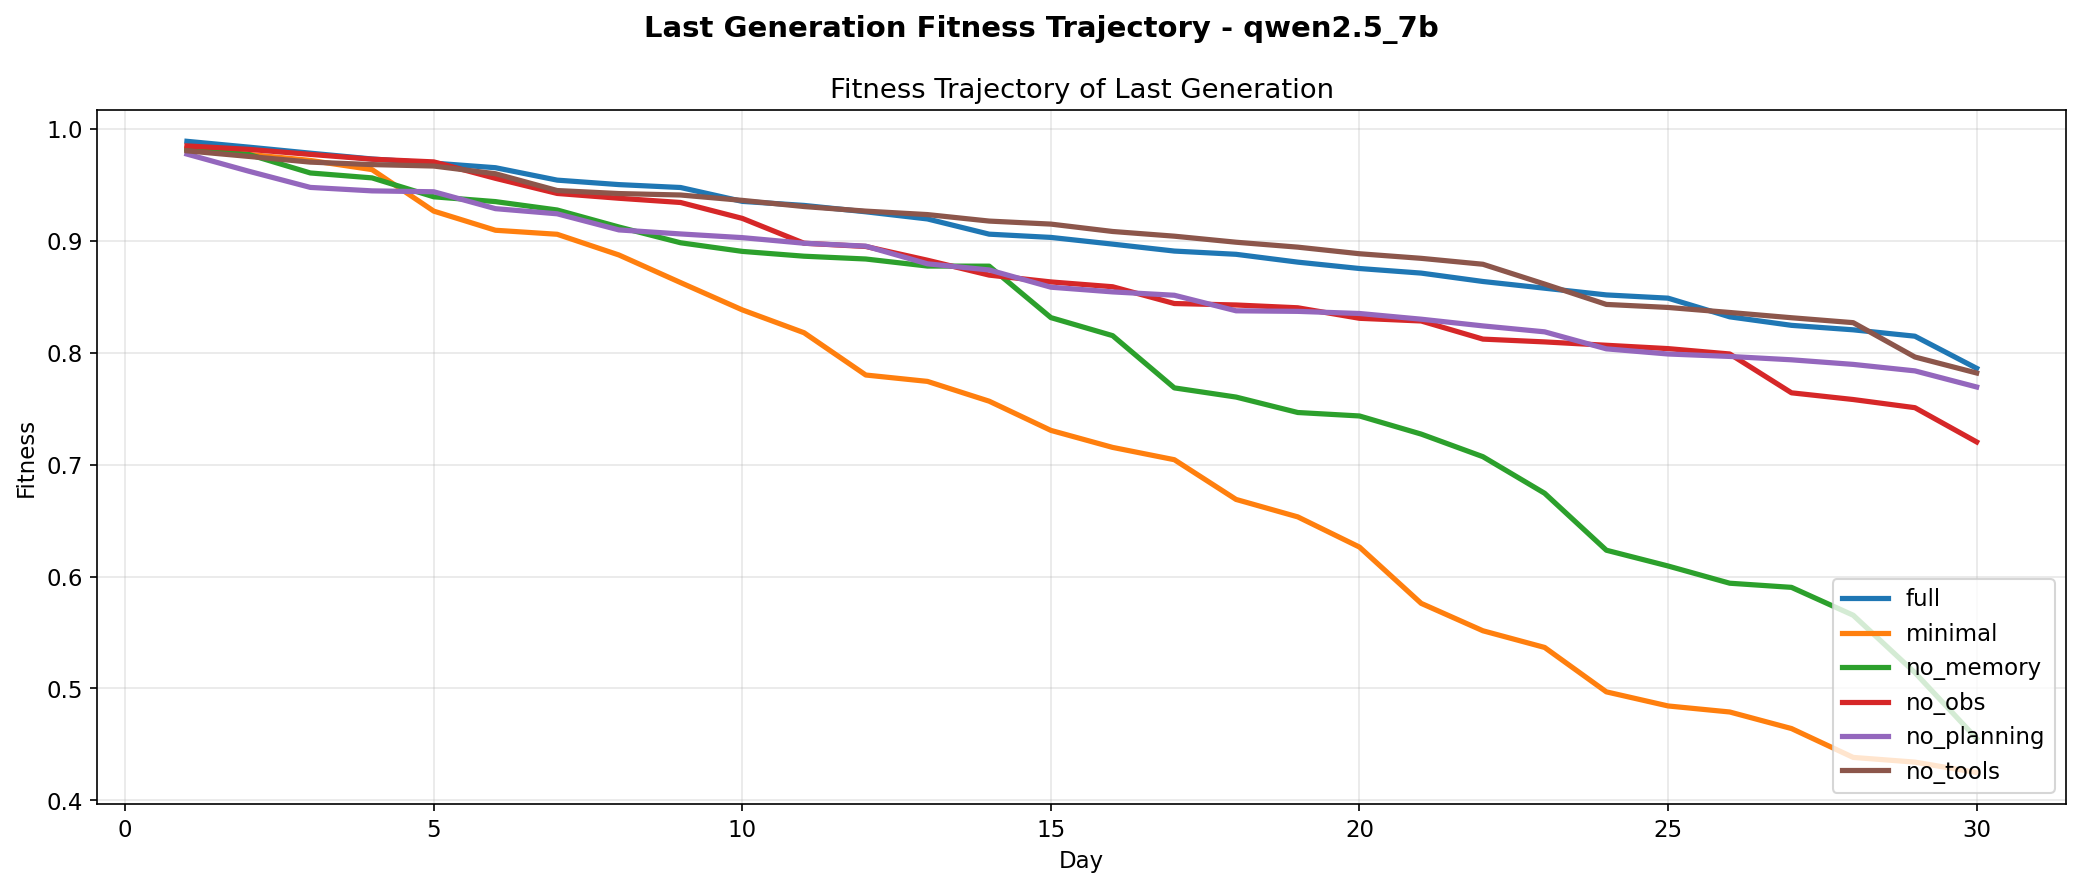
\includegraphics[width=\linewidth]{../plots/qwen2.5_7b/last_generation_trajectory.png}
        \caption{30-Day Trajectory (Qwen2.5 7B)}
        \label{fig:trajectory_7b}
    \end{minipage}\hfill
    \begin{minipage}{0.48\textwidth}
        \centering
        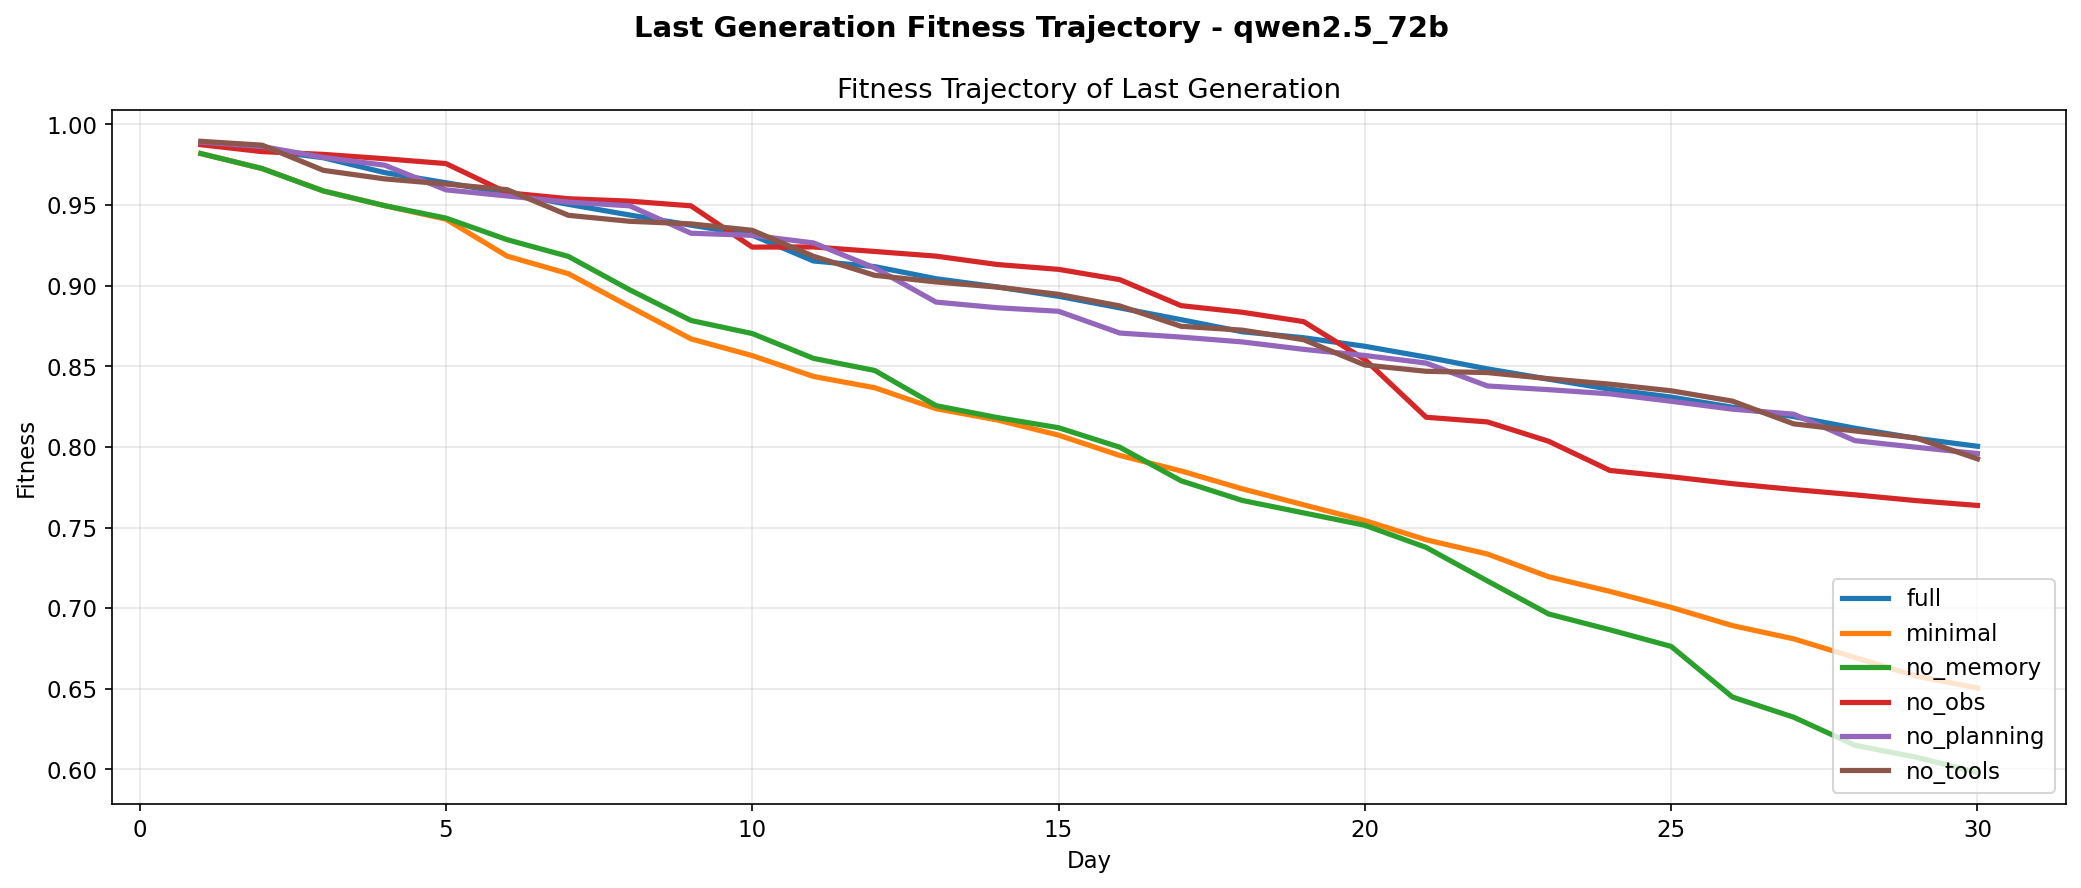
\includegraphics[width=\linewidth]{../plots/qwen2.5_72b/last_generation_trajectory.png}
        \caption{30-Day Trajectory (Qwen2.5 72B)}
        \label{fig:trajectory_72b}
    \end{minipage}
\end{figure}

\subsection{Computational Overhead: Token and Word Usage}
Evaluating cost (Figures \ref{fig:tokens_7b} and \ref{fig:tokens_72b}) shows that these represent raw total context provided by the API. Both models fundamentally overflow their respective context windows during a full 30-day run. The Memory Compaction module is thus required to maintain a functional context window. While the 72B model generally consumes a higher token count than the 7B model, the resulting depth of reasoning is critical for the superior performance seen in the \textit{Full} configuration.

\begin{figure}[H]
    \centering
    \begin{minipage}{0.48\textwidth}
        \centering
        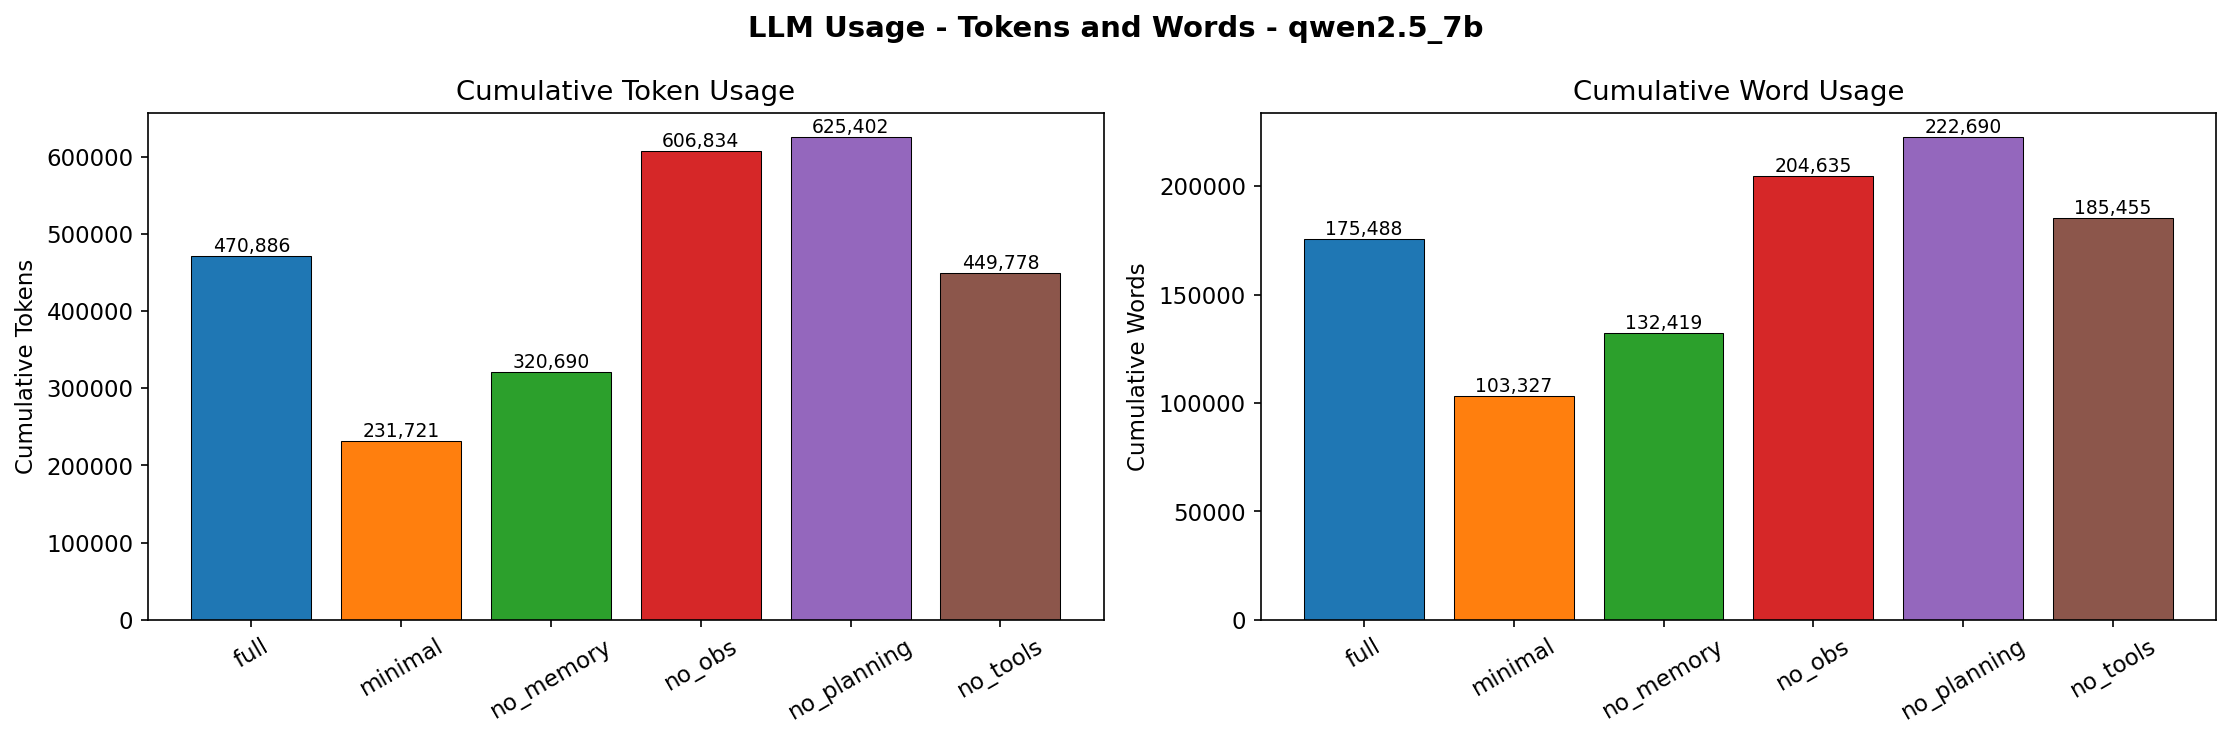
\includegraphics[width=\linewidth]{../plots/qwen2.5_7b/token_word_usage.png}
        \caption{Token and Word Usage (Qwen2.5 7B)}
        \label{fig:tokens_7b}
    \end{minipage}\hfill
    \begin{minipage}{0.48\textwidth}
        \centering
        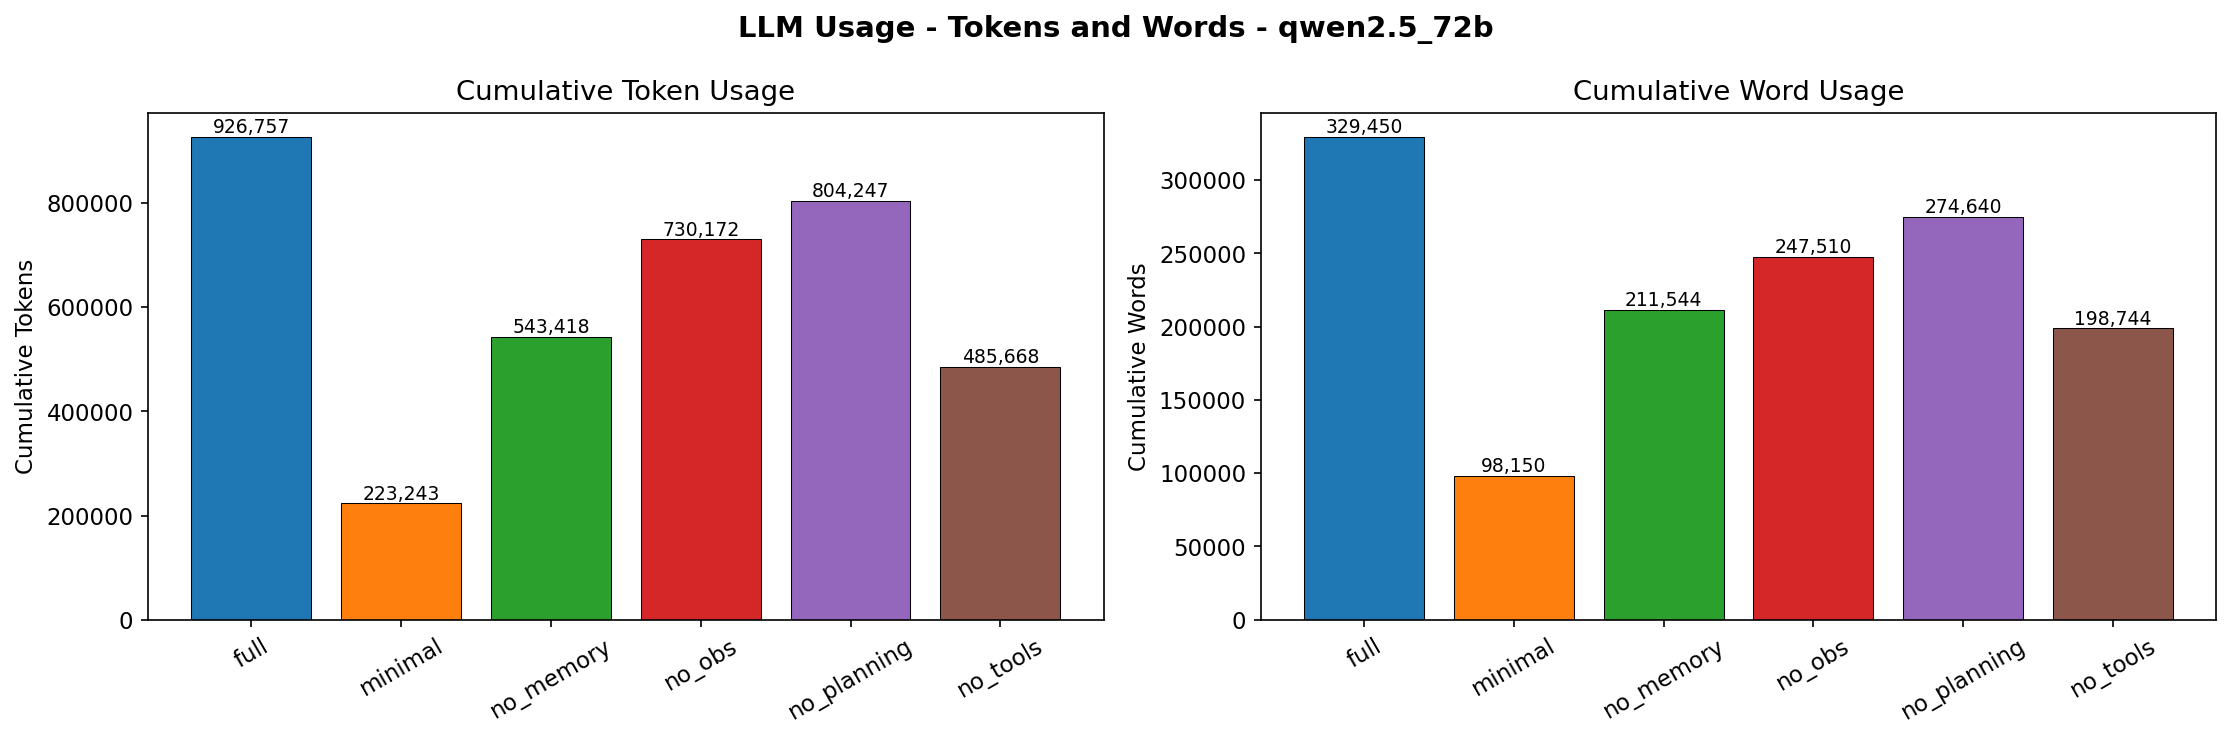
\includegraphics[width=\linewidth]{../plots/qwen2.5_72b/token_word_usage.png}
        \caption{Token and Word Usage (Qwen2.5 72B)}
        \label{fig:tokens_72b}
    \end{minipage}
\end{figure}

\section{Conclusion}
This study demonstrated that Large Language Models can act as effective autonomous agents within the high-dimensional and unpredictable domain of aquaculture management. The development of AquaLLM successfully bridged the gap between natural language reasoning and 3D agent-based biological simulations. Our results confirm that while a larger model scale, such as the 72B parameter variant, provides superior reasoning regarding biological causality and multi-objective optimization, these improvements are not currently proportional to the massive increase in computational overhead. The 7B model proved to be a surprisingly efficient alternative for basic management tasks, suggesting that for specific resource-constrained applications, smaller models with robust cognitive scaffolding may be more viable than simply increasing parameter counts.

However, several drawbacks in the current experimental scope must be acknowledged. Due to the significant computational cost of running local high-parameter inference alongside a complex physics simulation, our analysis was limited to five generational cycles and a single execution per configuration. This constraint prevents a full statistical validation of the agent's learning stability over long horizons. Furthermore, the virtual pond environment is inherently stochastic and chaotic, characterized by delayed biological feedback loops and non-linear hazard propagation. Given this complexity, we conclude that the "farmer" role in such a setup requires an even larger model scale or perhaps domain-specific fine-tuning to achieve a truly optimized equilibrium.

Ultimately, this project highlights that raw model scale cannot replace architectural necessity. Regardless of parameter count, the inclusion of memory compaction and tool-augmentation remains the most critical requirement for embodied agents. Without these modules, models of any size succumb to context overflow and mathematical hallucinations. Future work should focus on increasing the generational count to observe long-term optimization trends and exploring specialized training to help the LLM better navigate the chaotic trajectories of aquaculture ecosystems.

\section{Appendices}

\subsection{Code Design}
The codebase is separated into two primary functional domains:
\begin{itemize}
    \item \textit{Core Simulation (\texttt{/core}):} Logic for entities, physics, and behaviors.
    \item \textit{Agent Architecture (\texttt{/agent}):} Logic for memory, observation, and tools.
\end{itemize}
The implementation of the core simulation environment and the development of several cognitive modules (specifically the initial drafting of the system prompts and the logic for the Memory Compaction feature) were significantly accelerated through the use of Claude Code. This AI-assisted development workflow allowed for rapid iteration between the stochastic biological requirements of the simulation and the technical constraints of the LLM agent architecture.

\subsection{Workload Distribution}
I was the sole contributor to this project. All tasks were completed individually.

\subsection{System Prompt Engineering}
The agent is initialized with modular system templates:
\vspace{1em}
\textit{1. Overarching Objectives (\texttt{\_CORE\_TEMPLATE})}
\begin{lstlisting}
You manage an aquaculture fish pond. {days}d ${budget} budget. {fish} fish fixed.
There are {gens} generations total. Use previous generation results only as evidence for better decisions; do not experiment casually. The last generation is graded and is very important.
Best strategy: Gen-1 Day-0 should start with the cheapest valid conservative policy, then later generations should improve from evidence. A cheap baseline reveals what actually fails without wasting budget early.
This is a losing game: Fitness usually declines over time. Goal: prevent sharp Fitness drops while preserving Saving.
Fitness=0.55*Yield + 0.33*Saving + 0.12*Health. Saving is important. Over budget/all dead=Fitness 0.
Initial policy is extremely important. Prefer a conservative, affordable initial policy unless prior evidence clearly supports spending more.
Cost rule: smaller interval = more frequent = higher cost. Larger interval = cheaper. Smaller quantity/duration = cheaper. Larger quantity/duration = higher cost.
Valid ranges: food_interval 1-12, food_quantity 5-30, probiotic_interval 24-168, probiotic_quantity 1-4, oxygen_interval 1-20, oxygen_duration 1-4, locations 0-9.
Never recommend invalid values like probiotic_interval=12. Avoid food_interval=10 fixation.
Reflections are token-capped. Keep every reflection short: one concise lesson plus at most one param=value.
Only fish stats: health, fullness, immunity, oxygen. ALL intervals are HOURS. Output compact JSON only.
Locations: 0=Center 1=TL 2=TR 3=BL 4=BR 5=TC 6=BC 7=LC 8=RC 9=Random.
\end{lstlisting}

\textit{2. Reflection Protocol (\texttt{\_REFLECTION\_USAGE\_BLOCK})}
\begin{lstlisting}
Reflection types have different purposes and all reflections are token-capped, so keep them short:
- CHECKPOINT reflection: mid-generation review; use only for next-day adjustment in the current generation.
- WARNING reflection: urgent mid-generation warning; use only for next-day adjustment in the current generation. A warning often means spending/feeding/pumping too much is creating waste, pollutants, NH3, disease, parasites, or budget pressure. For WARNING reflections, first consider spending LESS: increase intervals, reduce quantity/duration, or move drops away from hazards. Do not automatically spend more unless the warning clearly says fish are starving or suffocating.
- END_GEN_REFLECTION: generation summary; use only to choose the next generation Day-0 initial policy.
- EARLY_QUIT_REFLECTION: failed-start summary; use only to avoid that bad initial policy on the restarted/next generation.
Do not confuse these. Mid-gen reflections guide tomorrow. End-gen and Early-Quit reflections guide the next initial policy. Reflection format should be short: reason; optional NEXT_START: param=value.
\end{lstlisting}

\textit{3. Chain-of-Thought Scaffolding (\texttt{\_PLANNING\_BLOCK} \& \texttt{\_COUNTER\_BLOCK})}
\begin{lstlisting}
Think briefly: Fitness drop mild or sharp? weakest stat? cheapest fix? budget? Which reflection type is present, and should it affect tomorrow or next generation Day-0? If WARNING reflection is present, ask whether overspending/pollution is the cause before spending more. Is candidate identical to CURRENT_POLICY? If identical, keep policy. JSON.
If reflection says exact param=value, use it only if valid, affordable, different from current policy, and appropriate for that reflection type.

Rules: mild decline + stats OK -> keep policy and save. sharp drop/stat<0.5 -> cheapest fix. WARNING reflection -> first suspect overspending, waste, pollutants, hazards, or budget pressure; spending less is often better. low_fullness->adjust food carefully; leftover food causes pollution. low_oxygen->oxygen_interval first, duration only if severe. low_immunity->probiotic sparingly; probiotic_interval cannot be below 24. hazards->move drops away/reduce food. over budget->increase oxygen_interval, reduce oxygen_duration, then increase food_interval.
\end{lstlisting}

\textit{4. Mathematical Grounding (\texttt{\_TOOLS\_BLOCK})}
\begin{lstlisting}
Cost/day: food=(24/food_interval)*food_quantity*$0.05; prob=(24/probiotic_interval)*probiotic_quantity*$0.75; O2=(24/oxygen_interval)*oxygen_duration*$2.50. Smaller interval costs more. Smaller quantity/duration costs less. Target average spend ${daily:.2f}/day. Use calculate_budget when changing.
\end{lstlisting}

\textit{5. Temporal Action Execution (\texttt{\_FIRST\_ROUND\_BLOCK} \& \texttt{\_ADJUST\_BLOCK})}
\begin{lstlisting}
Day0: initial policy matters most. If this is Gen-1, start with the cheapest valid conservative baseline unless it is obviously impossible. If this is Gen-2 or later, use END_GEN_REFLECTION and EARLY_QUIT_REFLECTION as evidence for the initial policy. Do not use CHECKPOINT/WARNING reflections as next-generation initial-policy rules unless the end-gen reflection repeats them. Do not default food_interval=10. Use prior BEST as baseline if shown. Output ONLY compact JSON with 9 policy fields, no fish_count.

Read observation and CURRENT_POLICY. Use CHECKPOINT/WARNING reflections for next-day adjustment only. For WARNING, prefer spending less unless fish are clearly starving/suffocating. Ignore END_GEN_REFLECTION/EARLY_QUIT_REFLECTION for same-day emergency changes unless they are restated as current evidence. If decline is mild, keep CURRENT_POLICY to preserve Saving. If sharp drop/stat<0.5, change the cheapest effective parameter. If candidate JSON equals CURRENT_POLICY, that is no change required. Output ONLY compact JSON: 9 fields + early_quit. No fish_count.
\end{lstlisting}

\textit{6. Proactive Abort Trigger (\texttt{\_EARLY\_QUIT\_BLOCK})}
\begin{lstlisting}
Early-Quit rule: Starting from Gen 3, if restart attempts remain, you may Early-Quit only after calling compare_day_fitness. Early-Quit is allowed only when current day Fitness is at least 5% below the average Fitness of the same day in previous generations. If Early-Quit is justified, output JSON with early_quit=true and keep policy fields unchanged.
\end{lstlisting}

\begin{thebibliography}{00}
\bibitem{urbanova2023} P. Urbanova et al., ``Agent Based Modeling of Fish Shoal Behavior,'' \textit{LNCS}, pp. 3--13, 2023.
\bibitem{hou2023} H. Hou et al., ``An Environmental Impact Assessment of Largemouth Bass Aquaculture,'' \textit{Sustainability}, 2023.
\bibitem{park2023} J. S. Park et al., ``Generative Agents: Interactive Simulacra of Human Behavior,'' \textit{Proc. UIST '23}, 2023.
\bibitem{wang2023} G. Wang et al., ``Voyager: An Open-Ended Embodied Agent with Large Language Models,'' \textit{arXiv:2305.16291}, 2023.
\end{thebibliography}

\end{document}